\subsection{Mathematische Formeln}

\begin{frame}[fragile]{\subsecname}
    Mathematische Formeln können auf verschiedene Arten und Weisen im so genannten \alert{Math Mode}
    gesetzt werden:
    \begin{itemize}
        \item \emph{Inline Math}: Innerhalb von Fließtext mittels \code{$...$}:
            \example*{examples/inline_math.tex}
        \item \emph{Display Math}: Abgesetzt in einer separaten Zeile mittels \code{\[...\]}:
            \example*{examples/display_math.tex}
    \end{itemize}
\end{frame}

\begin{frame}[fragile]{Indizes und Exponenten}
    \begin{itemize}
        \item Indizes:
            \example*{examples/indices.tex}
            Beachte: Für Indizes mit mehr als einem Zeichen muss der Index in geschweifte Klammern
            gesetzt werden: \code{v_{i-1}}.
        \smallskip
        \item Exponenten:
            \example*{examples/exponents.tex}
            Beachte: Wie bei Indizes müssen mehrere Zeichen in geschweifte Klammern gesetzt werden:
            \code{n^{k+1}}.
    \end{itemize}
\end{frame}

\begin{frame}[fragile]{Mehrzeilige Formeln}
    \begin{itemize}
        \item Für mehrzeilige Formeln bieten sich Umgebungen wie \texttt{align} an:
            \example*{examples/align.tex}
        \item Die Zeilen werden dabei anhand der \code{&} ausgerichtet.
        \item Nummerierung kann mit \code{\nonumber} pro Zeile ausgeschaltet werden -- oder man
            nutzt \texttt{align*} statt \texttt{align}.
        \item Andere nützliche Umgebungen sind \texttt{equation}, \texttt{gather}, \texttt{array},
            \texttt{multiline}.
        \item Diese Umgebungen werden vom Paket \texttt{amsmath} bereitgestellt, welches daher bei
            Bedarf in der Präambel eingebunden werden muss:
            \begin{center}
                \code{\usepackage{amsmath}}
            \end{center}
    \end{itemize}
\end{frame}

\begin{frame}[fragile,t]{Mathematische Symbole}
    \begin{itemize}
        \item Das Paket \texttt{amssymb} enthält weitere mathematische Symbole:
            \begin{center}
                \code{\usepackage{amssymb}}
            \end{center}
        \item Falls man einen Befehl für ein bestimmtes mathematisches Symbol sucht, hilft der Dienst
            \href{http://detexify.kirelabs.org/classify.html}{\alert{Detexify}} weiter:
            \begin{center}
                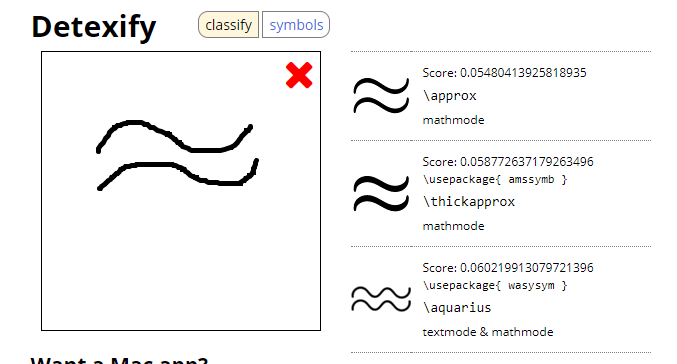
\includegraphics[keepaspectratio,width=8cm]{\thistopic/detexify.png}
            \end{center}
    \end{itemize}
\end{frame}
